\chapter{Future Plan}\label{C:future} 

This final chapter will outline the work that is yet to be completed for this project, and how we plan complete it. It will also discuss how we plan to evaluate this system once this future work has been completed, outlining the changes to the evaluation that have come about since the project proposal. Finally this chapter will then present the project timeline for the remaining work and evaluation, breaking down this work into discrete blocks of time. 

\section{Work to be Completed}\label{S:work_remaining}

As discussed in \Cref{S:system}, there are 3 main segments of work in this project. The first segment of work was the PWM generator, which has been outlined in \Cref{S:pwm_gen} and has already been completed. The next two section were the specification and selection of the required sensing elements, and then the implementation of the control system that will make this project functional.\\

To complete the specification and selection of the sensing elements, a large amount of background research will need to be completed. This research will include the identifying of various ways that the inductor current ripple can be measured, as well as defining the required specifications of the sensors based on the system requirements. Once this research has been completed and components have been selected, it will be important to evaluate the functionality of the components, to verify that they do meet the required specifications. Finally once the sensing elements have been selected and tested, the creation of a printed circuit board (PCB) to hold the PWM generator, sensing elements, and buck converter will be completed. This PCB will be the final physical artefact that is created from this project. \\

Once this physical artefact has been generated, the only section left to be completed is the projects control system. This control system will be responsible for regulating both the inductor ripple current and the buck converter output voltage. To be able to successfully implement this section of the project I will again need to perform a section of background research. This research will inform the design and implementation of this controller within the microcontroller, helping to select the controller architecture and structure. Once the controller design has been specified, it will need to be implemented in software on the microcontroller, allowing for time to test the implementation. 

\section{System Evaluation}


    The evaluation of this system has not changed substantially since the project proposal, and is still based upon meeting the following selection of specifications. 
    
    However, the evaluation of the system will now be conducted using a range of load resistances, evaluating its performance with 10$\Omega$, 15$\Omega$, and 20$\Omega$ output loads, using a constant supply voltage of 12V DC.

\begin{itemize}
	\item The buck converter will be able to take input voltages up to 12V DC
	
	\item The buck converter must maintain the basic functionality outlined in \cref{E:V_out}

	\item The buck converter will have an output voltage range between 3V and 10V DC
	
	\item The output voltage accuracy will be within $\pm 5\%$ of the target output voltage

	\item The user will be able to define the inductor ripple between 20\% and 50\%
	
	\item The inductor ripple accuracy will be within $\pm 5\%$ of the defined inductor ripple
	
	\item The buck converter will have a switching frequency range of 1k$Hz$ to 100k$Hz$

	\item The control system will have no steady state error

\end{itemize}

Since all of these evaluation metrics are highly qualitative, the evaluation of the final artefact will consist of a series of tests that will look to confirm the systems ability to achieve each of theses requirements.  

\section{Project Timeline}

The Gantt chart in \Cref{F:gantt} directly relates the remaining work set out in \Cref{S:work_remaining} to the time remaining for the project. For both the sensing element design and the control system, we believe that a large amount of background research will need to be completed before work is able to commence. This background research will inform and help reduce the time require to effectively design these sections. we plan to have all of the implementation and evaluation of the system completed before the end of the mid trimester break, as this will allow for a large amount of report writing time.

\begin{figure}[H]
    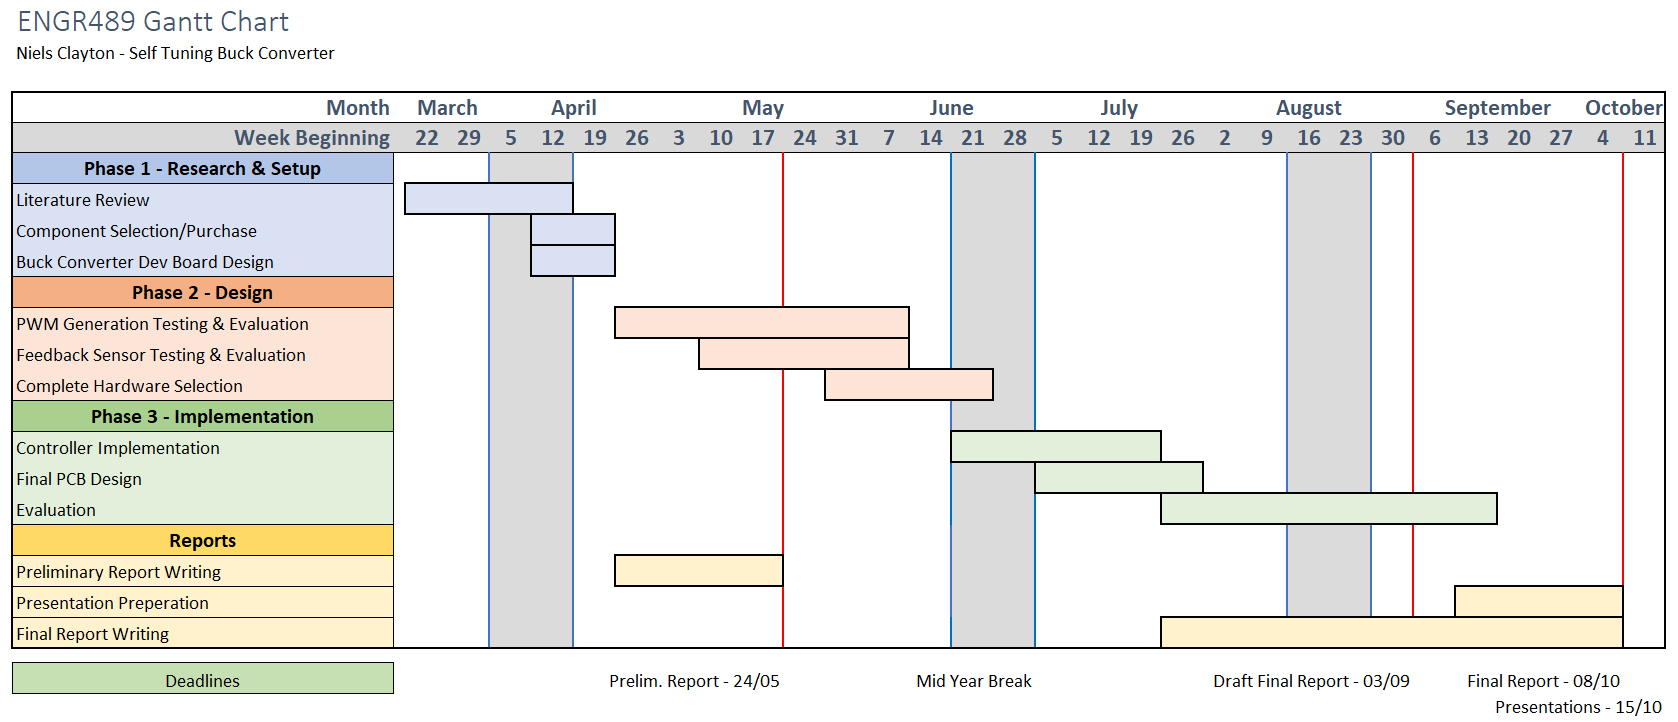
\includegraphics[width = 1\textwidth]{gantt.png}
    \caption{Proposed project timeline}
    \label{F:gantt}
\end{figure}


\section*{Feedback}\label{S:feedback} 

At this stage in the project I have a very clear idea as to what I am planning to, and how I am planning to get there. I would also greatly appreciate all feedback that can be provided on this report, so that I can implement the changes in my final report. I would greatly appreciate it if It would be possible to organise an in person meeting with my markers to discuss this report and project. 